% esta si 
\documentclass{article}
\usepackage[utf8]{inputenc}
\usepackage[spanish]{babel}
\usepackage{graphicx, graphics, float, fancyhdr, titling}
\usepackage{listings, subcaption}
\usepackage[a4paper, total={6in, 9.5in}]{geometry}
\usepackage{hyperref}

\setcounter{secnumdepth}{-2}

\renewcommand{\footrulewidth}{0.4pt}
\title{

\includegraphics[width=1.75in]{imagenes/UGR-Logo.png} \\
\vspace*{1in}
\textbf{Práctica 4, Sesión 2} \\
Seguridad en Sistemas Operativos \\
\vspace*{0.5in}}
\author{Andrés Merlo Trujillo \\
\vspace*{0.5in} \\
E.T.S. de Ingenierías Informática y de Telecomunicación \\
\textbf{Universidad de Granada}} \date{\today}
%\date{}
\hypersetup{
    colorlinks=true,
    linkcolor=black,
}

\renewcommand\maketitlehooka{\null\mbox{}\vfill}
\renewcommand\maketitlehookd{\vfill\null}


\begin{document}
\begin{titlingpage}
\maketitle
\end{titlingpage}

\newpage

\tableofcontents

\newpage

\pagestyle{fancy}
\fancyhead[L]{Andrés Merlo Trujillo}
\fancyhead[R]{Seguridad en Sistemas Operativos}
%\addcontentsline{toc}{section}{Ejercicio 1}
%\section{Ejercicio 1}
%\begin{figure}[H]
%    \centering
%    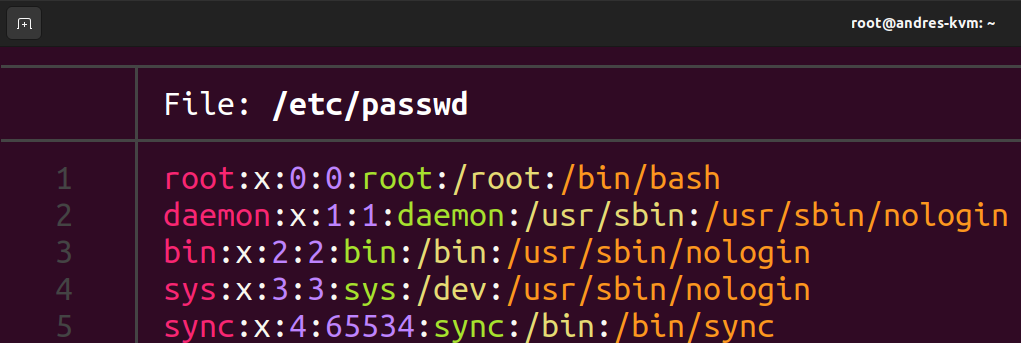
\includegraphics[width=\textwidth]{imagenes/passwdfile.png}
%\end{figure}

\section{Ejercicio 1}

Primero hay que saber la version exacta del kernel para poder instalar el paquete \verb|linux-headers|, para ello, se usa el comando \verb|uname -r|:

%salida comando
\begin{figure}[H]
    \centering
    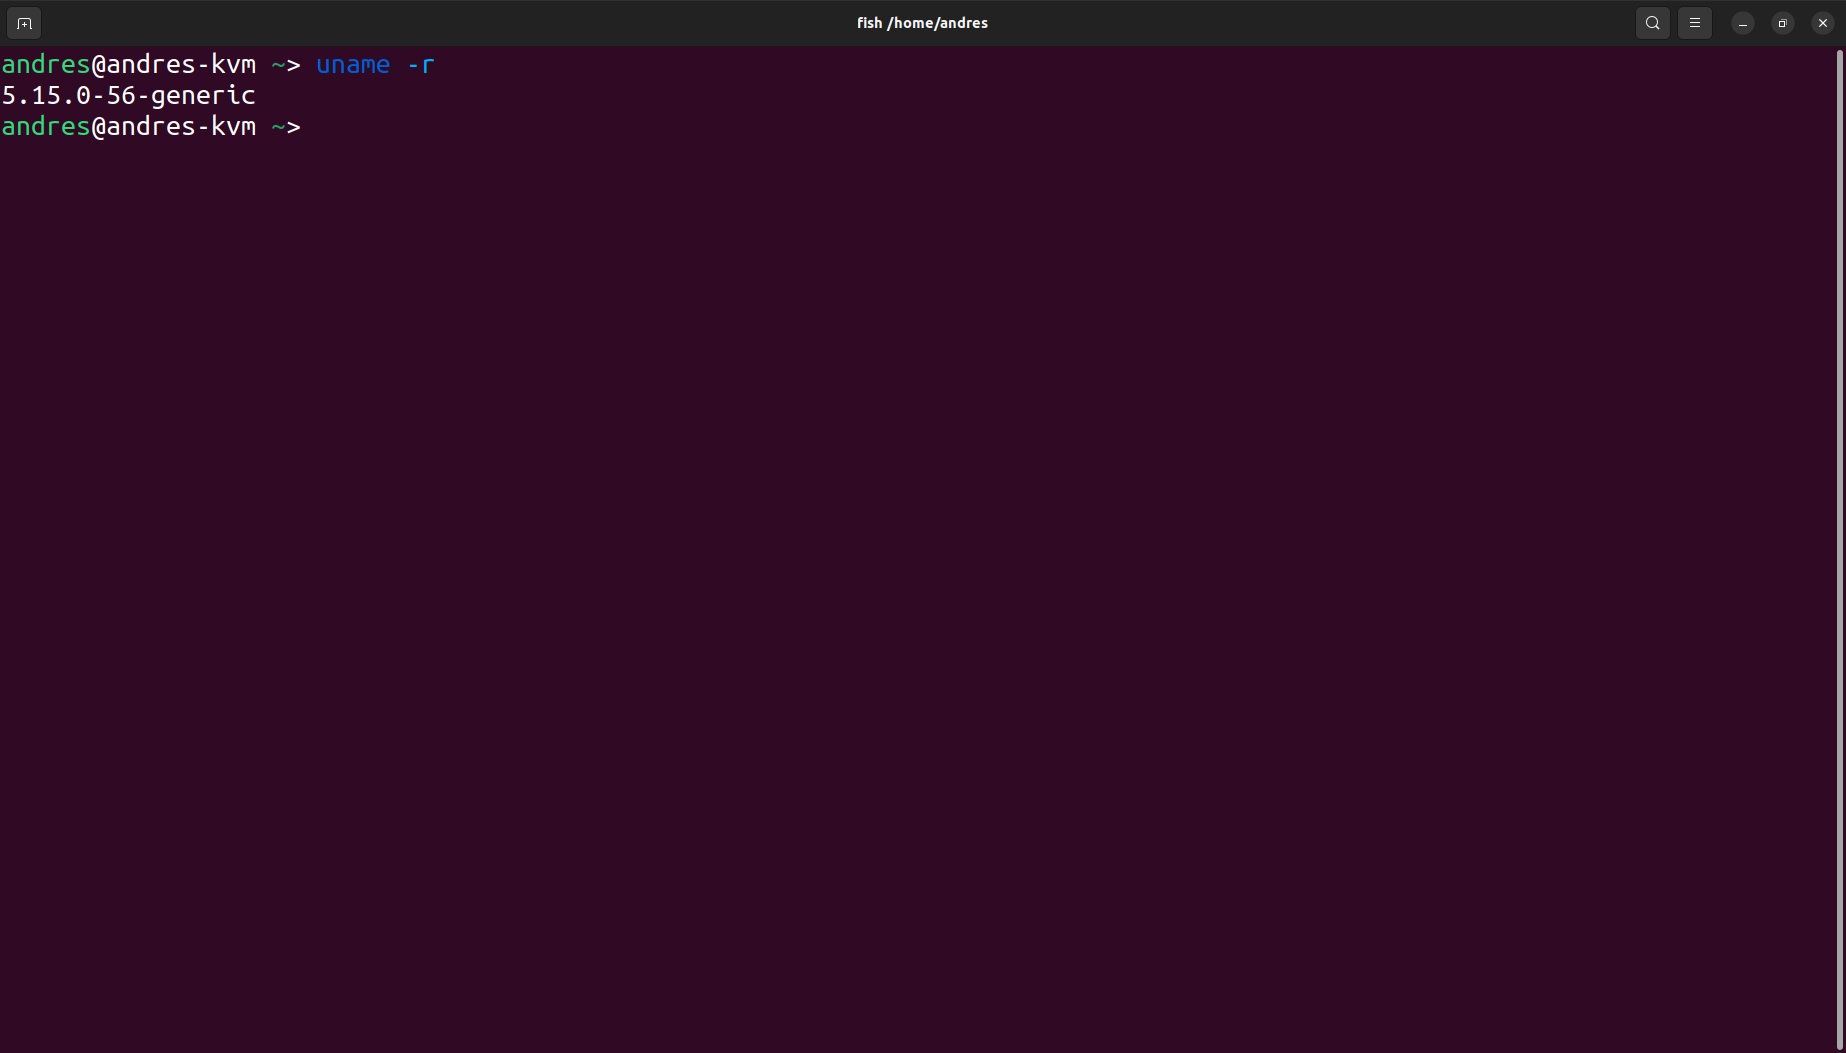
\includegraphics[width=0.6\textwidth]{imagenes/Captura desde 2022-12-06 11-37-14.png}
    \caption{Version del kernel que está usando mi distribucion.}
\end{figure}

Ahora lo que hay que hacer es instalar \verb|LiME| siguiendo las instrucciones proporcionadas en el guion de practicas. Una vez instalado, como es en maquina local, se ejecuta el comando:

\noindent
\verb|insmod lime-5.15.0-56-generic.ko path=/home/usuario/evidencias/volcado101 format=raw|

%foto
\begin{figure}[H]
    \centering
    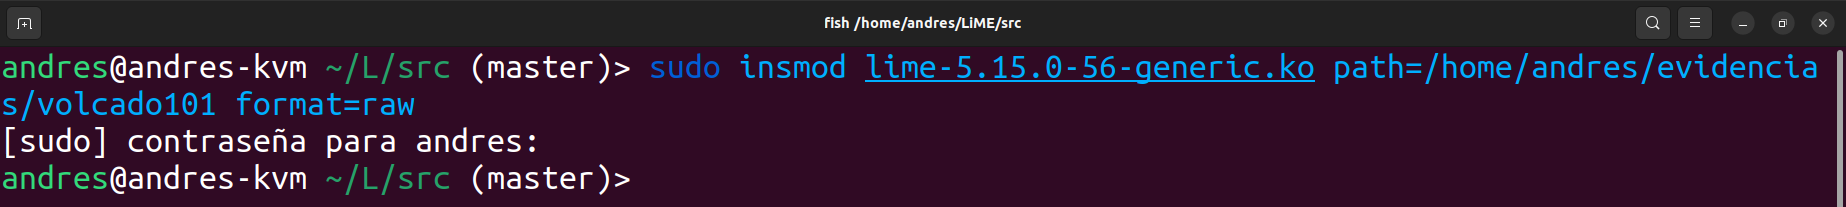
\includegraphics[width=\textwidth]{imagenes/Captura desde 2022-12-06 11-41-59.png}
    \caption{Volcado de memoria realizado.}
\end{figure}

Y ahora si nos vamos al directorio \textit{evidencias} deberia aparecer lo siguiente:

%foto del archivo
\begin{figure}[H]
    \centering
    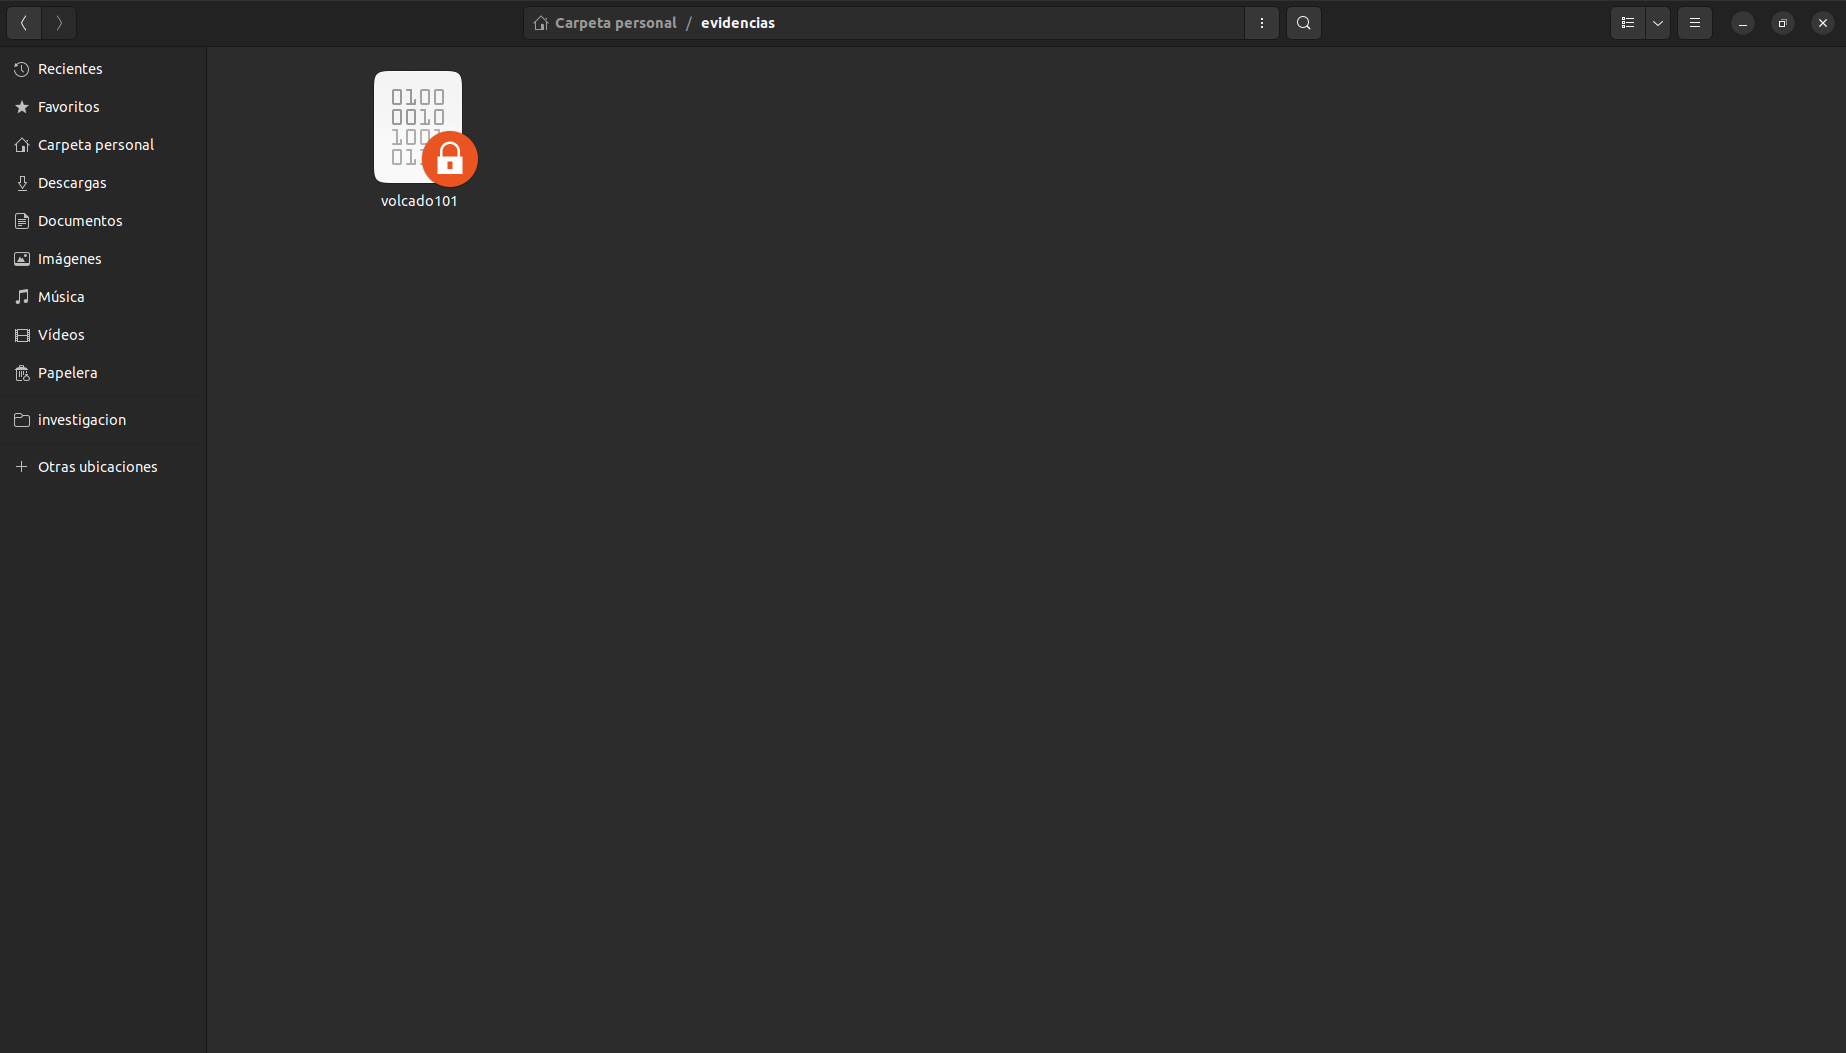
\includegraphics[width=\textwidth]{imagenes/Captura desde 2022-12-06 11-42-47.png}
    \caption{Volcado de memoria realizado correctamente.}
\end{figure}

\newpage
\section{Ejercicio 2}

Antes de nada hace falta instalar \verb|volatility| y descargarse la imagen RAM de PRADO.

\subsection{a) ¿A qué sistema operativo corresponde la imagen?}

Primero, para comprobar si usa Linux, se usa el comando \verb|strings memory.img | grep -i "Linux version" | uniq|, en caso de no devolver nada, es otro sistema operativo, seguramente Windows.

%foto para windows
\begin{figure}[H]
    \centering
    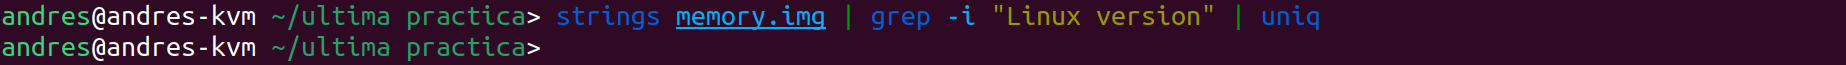
\includegraphics[width=\textwidth]{imagenes/Captura desde 2022-12-06 12-56-51.png}
    \caption{salida para un SO distinto de linux.}
\end{figure}

En cambio, con la imagen del ejercicio anterior (Linux) sale lo siguiente:

%foto de la slaida
\begin{figure}[H]
    \centering
    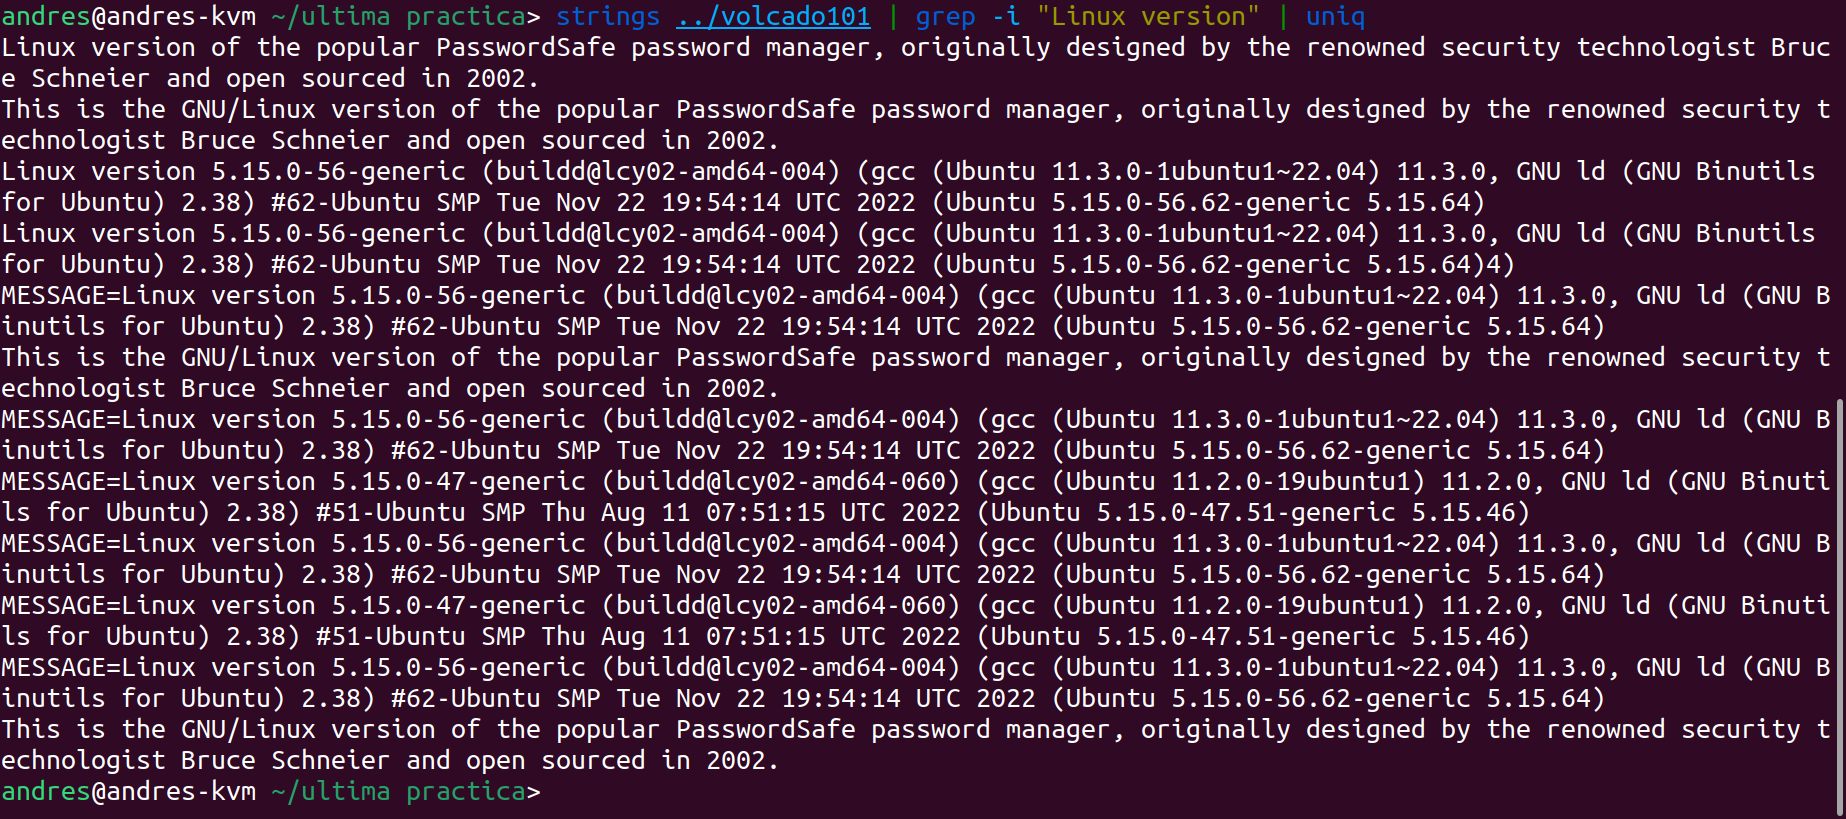
\includegraphics[width=\textwidth]{imagenes/Captura desde 2022-12-06 12-56-51-linux.png}
    \caption{en el volcado de memoria de Ubuntu sí aparecen referencias.}
\end{figure}


Y ahora, usando el comando \verb|vol.py -f memory.img imageinfo| se puede intuir que sistema operativo utiliza:

%foto
\begin{figure}[H]
    \centering
    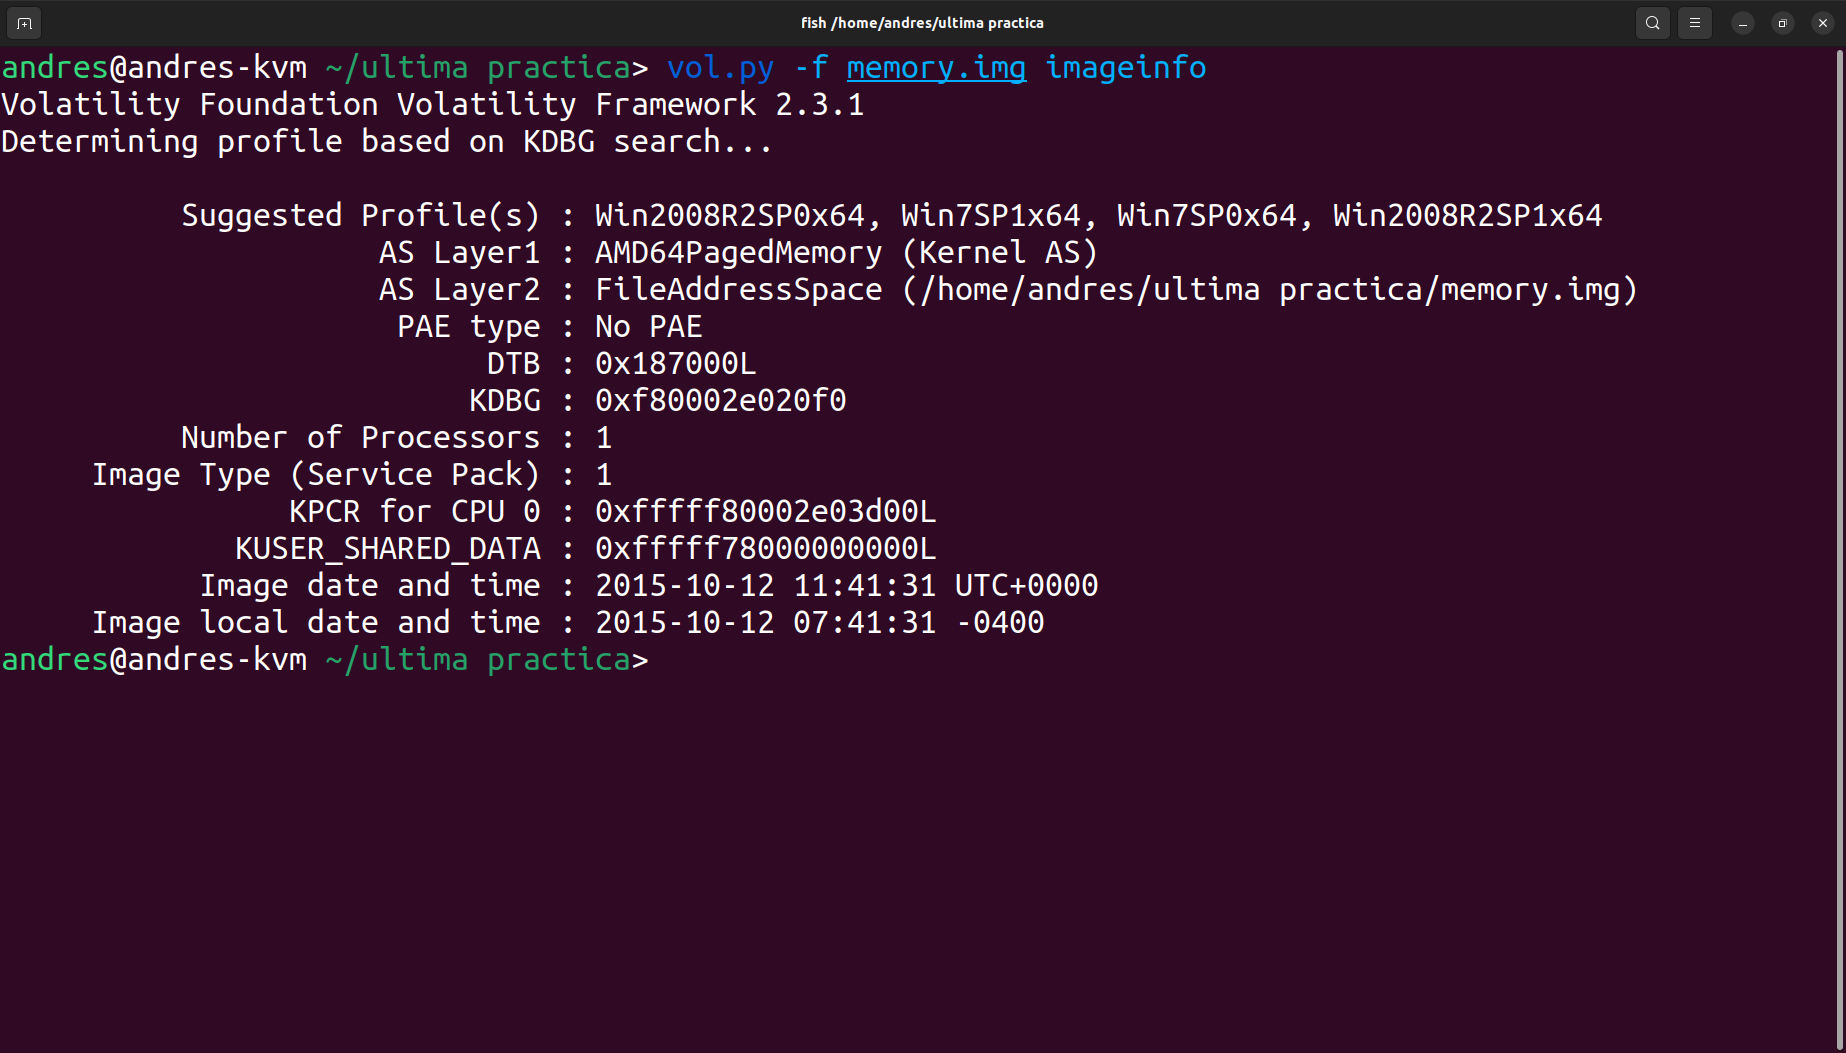
\includegraphics[width=\textwidth]{imagenes/Captura desde 2022-12-06 12-36-39.png}
    \caption{Salida del comando.}
\end{figure}

Como se puede ver, está usando Windows y por los perfiles sugeridos, parece ser que está usando Windows 7 o Windows Server 2008.

\subsection{b) Listar los procesos en ejecución en el momento de la adquisición.}

Usando la orden \verb|vol.py -f memory.img --profile=Win7SP1x64 pslist| se puede obtener esa informacion:

%foto de eso
\begin{figure}[H]
    \centering
    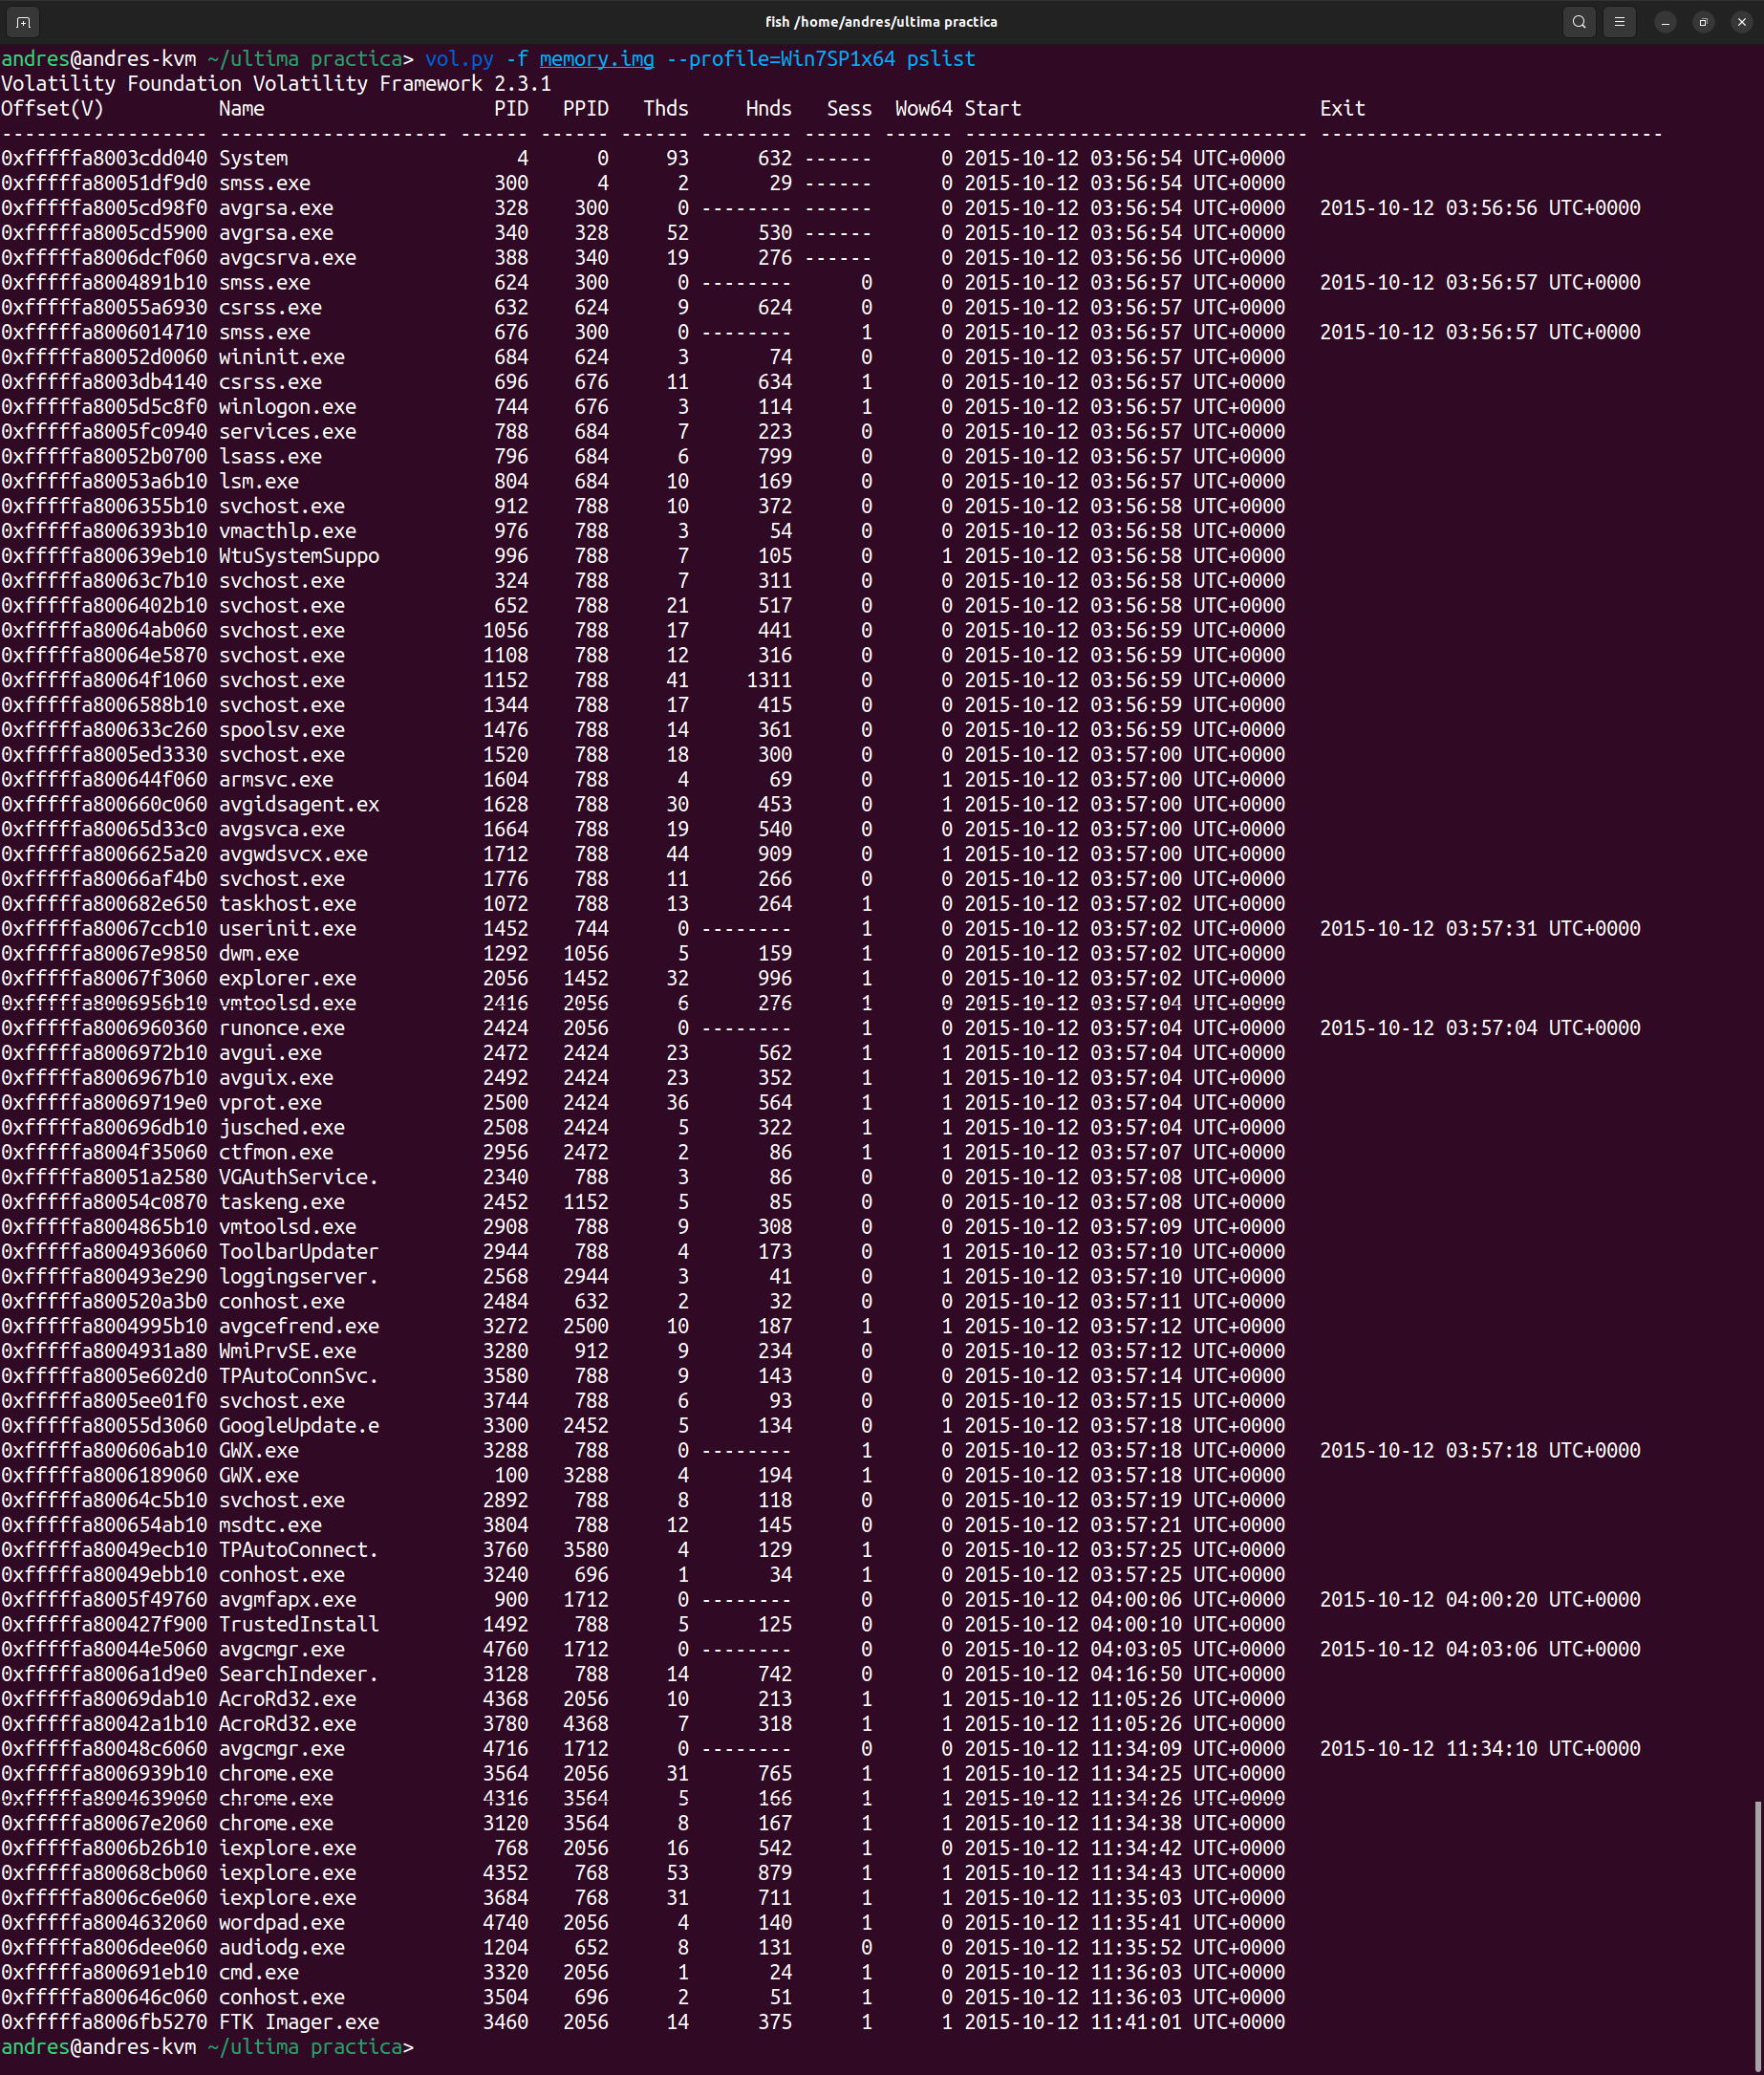
\includegraphics[width=\textwidth]{imagenes/pslist.png}
    \caption{Procesos en ejecucion en el momento de realizar el volcado de memoria.}
\end{figure}

\newpage
\subsection{c) Basado en el apartado b), ¿qué navegador se estaba usando en el momento de la adquisición?}

Basandome en la salida del comando anterior, se puede ver que se estaba eejcutando \verb|chrome.exe|.

%foto anterior recortada
\begin{figure}[H]
    \centering
    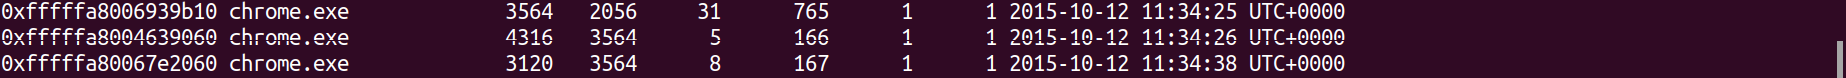
\includegraphics[width=\textwidth]{imagenes/pslist-1.png}
    \caption{\texttt{chrome.exe} en ejecución.}
\end{figure}

\subsection{d) ¿Cuál era el identificador de dicho proceso?}

El identificador se puede ver en la tercera columna, tienen el identificador 3564, 4316 y 3120.
\subsection{e) ¿Qué aplicación se utilizó para realizar la adquisición?}
El ultimo proceso de todos de la salida del comando anterior muestra que es FTK Imager.

%foto de eso
\begin{figure}[H]
    \centering
    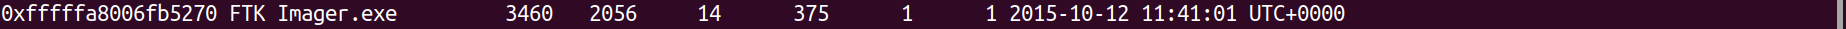
\includegraphics[width=\textwidth]{imagenes/pslist-2.png}
    \caption{FTK Imager en ejecucion para crear la imagen de la RAM.}
\end{figure}
\subsection{f) Mostrar las conexiones de red.}
Para obtener las conexiones de red se usa el comando:

\verb|vol.py -f memory.img --profile=Win7SP1x64 netscan|.

%foto
\begin{figure}[H]
    \centering
    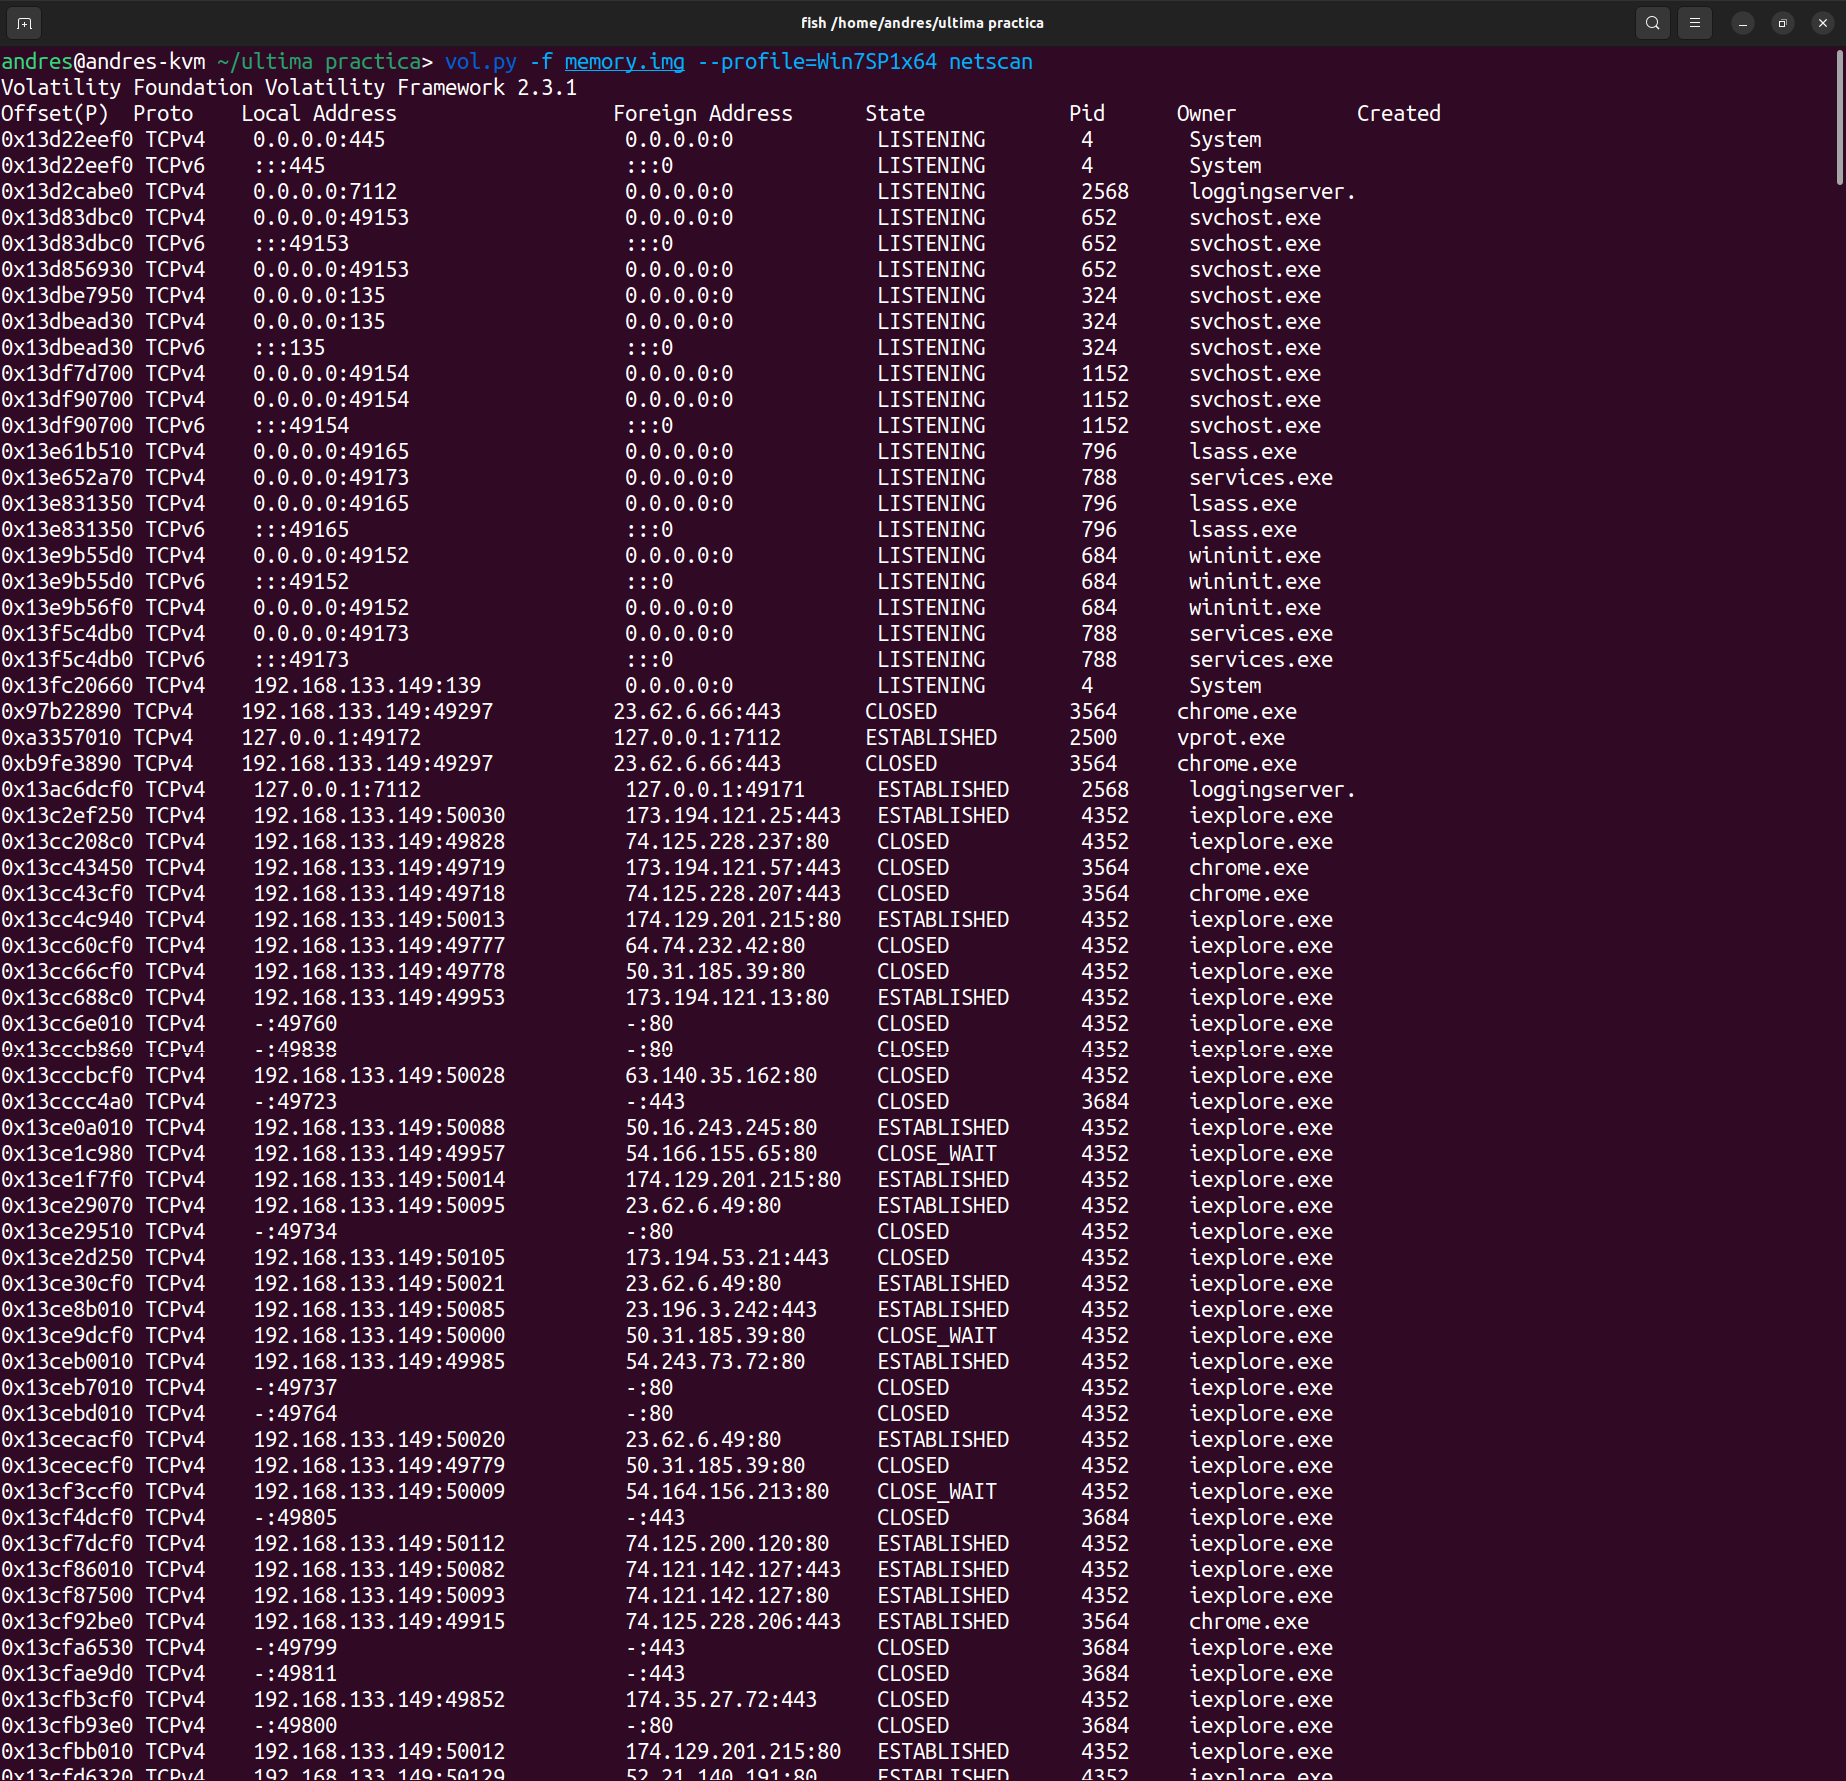
\includegraphics[width=0.8\textwidth]{imagenes/netscan.png}
    \caption{algunas conexiones que tenia ordenador.}
\end{figure}
\subsection{g) ¿A qué dirección IP estaba conectado Chrome cuando se realizó la adquisición?}

Se puede pasar por un \verb|grep| el comando anterior para obtener de forma rápida las direcciones IP. El comando quedaría así: \texttt{vol.py -f memory.img --profile=Win7SP1x64 netscan | grep ``chrome.exe''}.

%foto
\begin{figure}[H]
    \centering
    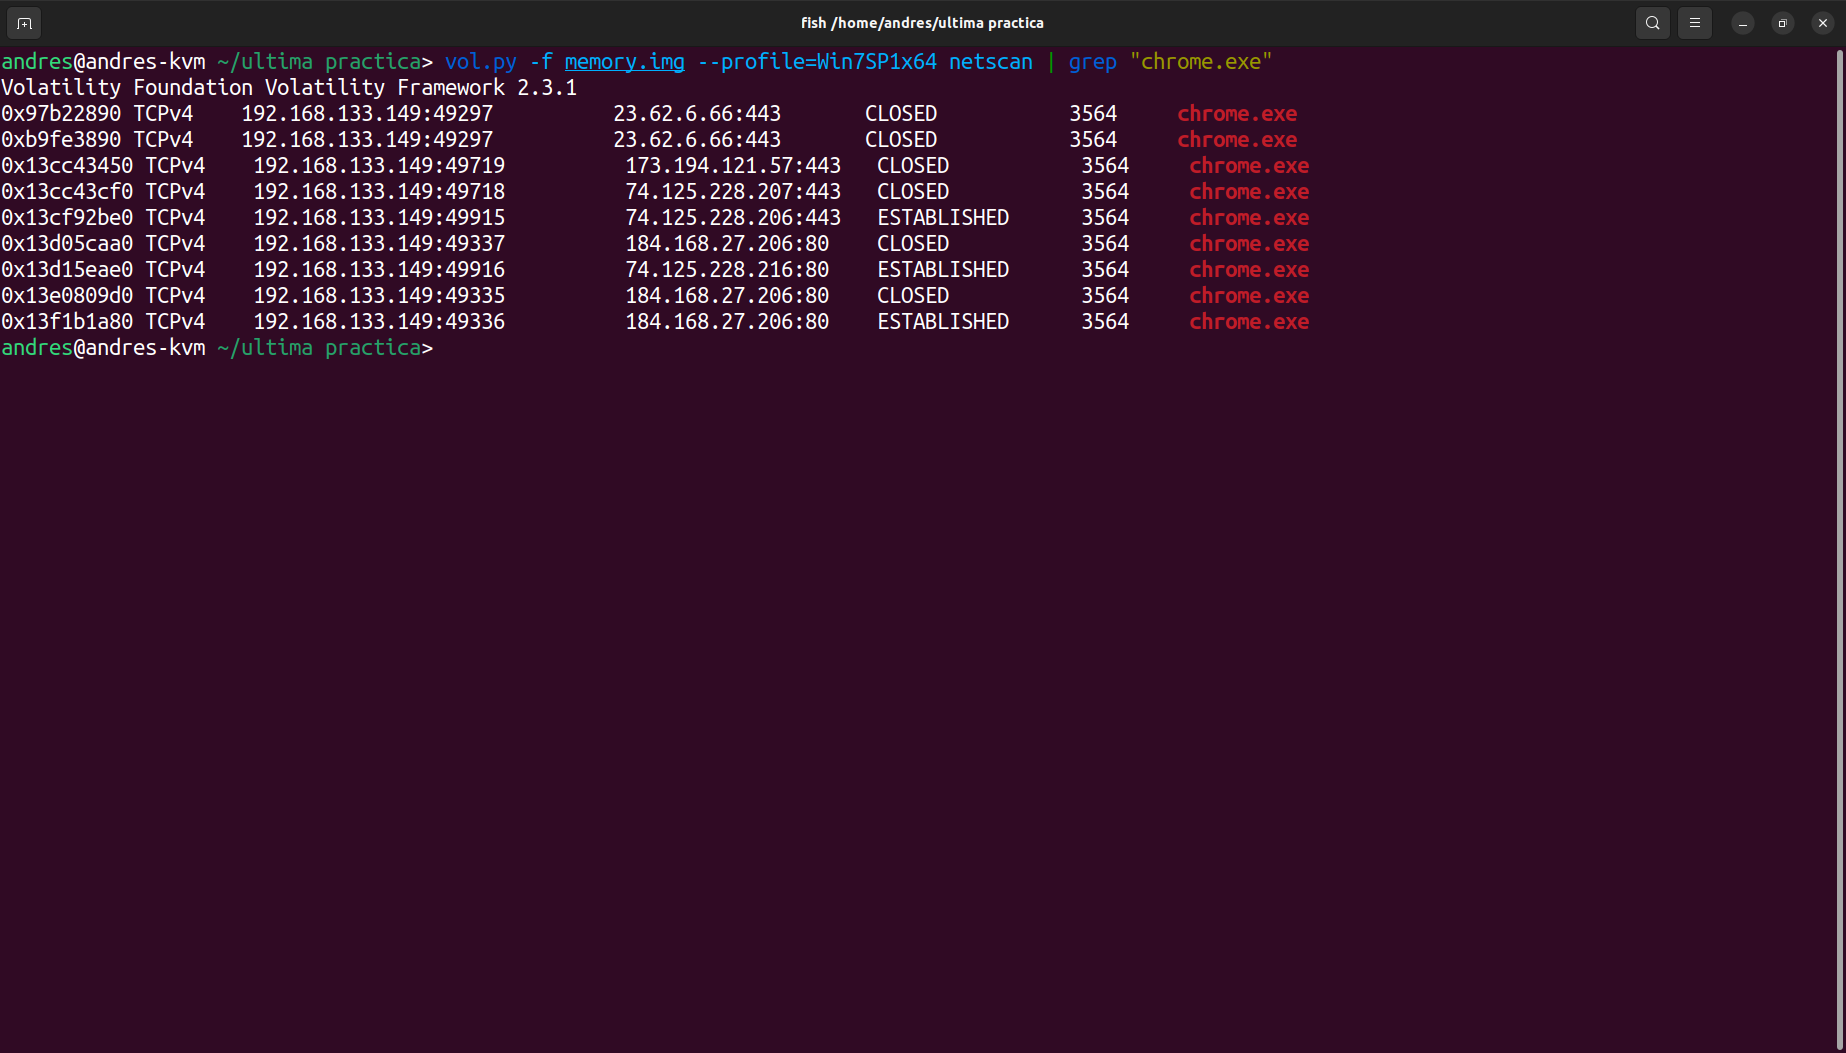
\includegraphics[width=\textwidth]{imagenes/Captura desde 2022-12-07 10-17-28.png}
    \caption{Conexiones abiertas por Chrome.}
\end{figure}

Por tanto, las conexiones que tenia abiertas eran la de \textbf{74.125.228.206:443}, \textbf{74.125.228.216:80} y \textbf{184.168.27.206:80}.

\end{document}
